\documentclass[border=4pt]{standalone}
\usepackage{tikz}
\usetikzlibrary{arrows,arrows.spaced,positioning}
\begin{document}
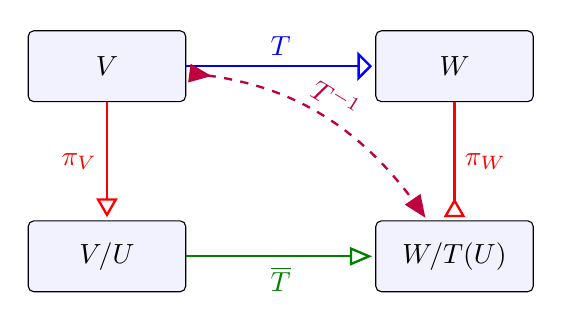
\begin{tikzpicture}[
  node distance=15mm and 24mm,
  object/.style={draw,rounded corners=2pt,minimum width=20mm,minimum height=9mm,fill=blue!5},
  map/.style={line width=.85pt}
]
  \node[object] (V) {$V$};
  \node[object,right=of V] (W) {$W$};
  \node[object,below=of V] (Q) {$V/U$};
  \node[object,right=of Q] (R) {$W/T(U)$};

  \draw[map,blue,-{spaced open triangle 90}]
    (V) -- node[above] {$T$} (W);
  \draw[map,red,-{spaced open triangle 60}]
    (V) -- node[left] {$\pi_V$} (Q);
  \draw[map,red,-{spaced open triangle 60 reversed}]
    (W) -- node[right] {$\pi_W$} (R);
  \draw[map,green!50!black,-{spaced open triangle 45}]
    (Q) -- node[below] {$\overline T$} (R);
  \draw[map,dashed,purple,{spaced triangle 45 reversed}-{spaced triangle 45}]
    (V) to[bend left=24] node[above,sloped] {$T^{-1}$} (R);
\end{tikzpicture}
\end{document}
